\documentclass{tufte-handout}

%\geometry{showframe}% for debugging purposes -- displays the margins

\usepackage{amsmath}

% Set up the images/graphics package
\usepackage{graphicx}
\setkeys{Gin}{width=\linewidth,totalheight=\textheight,keepaspectratio}
\graphicspath{{graphics/}}

\title{Writing Sample - Buffon's Needle Problem}
\author{Christian Jackson}
\date{}  % if the \date{} command is left out, the current date will be used

% The following package makes prettier tables.  We're all about the bling!
\usepackage{booktabs}

% The units package provides nice, non-stacked fractions and better spacing
% for units.
\usepackage{units}

% The fancyvrb package lets us customize the formatting of verbatim
% environments.  We use a slightly smaller font.
\usepackage{fancyvrb}
\fvset{fontsize=\normalsize}

% Small sections of multiple columns
\usepackage{multicol}

% Provides paragraphs of dummy text
\usepackage{lipsum}

% These commands are used to pretty-print LaTeX commands
\newcommand{\doccmd}[1]{\texttt{\textbackslash#1}}% command name -- adds backslash automatically
\newcommand{\docopt}[1]{\ensuremath{\langle}\textrm{\textit{#1}}\ensuremath{\rangle}}% optional command argument
\newcommand{\docarg}[1]{\textrm{\textit{#1}}}% (required) command argument
\newenvironment{docspec}{\begin{quote}\noindent}{\end{quote}}% command specification environment
\newcommand{\docenv}[1]{\textsf{#1}}% environment name
\newcommand{\docpkg}[1]{\texttt{#1}}% package name
\newcommand{\doccls}[1]{\texttt{#1}}% document class name
\newcommand{\docclsopt}[1]{\texttt{#1}}% document class option name

\begin{document}

\maketitle% this prints the handout title, author, and date
%\small
%\printclassoptions
\vspace{8px}
\noindent In 18th century France, the Count of Buffon was standing on a floor made of parallel strips of wood. He accidentally dropped a needle and it happened to land in such a way that it overlapped one of the lines on the floor. The Count became curious about the probability of such an event occurring. The calculation of this probability is Buffon's Needle Problem.
\begin{marginfigure}[-.1in]
\centering
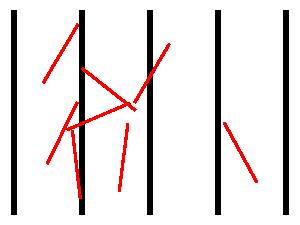
\includegraphics{ex}
\caption{An example of 8 needles lying on Buffon's floor. Some needles cross the edges of the floorboards and some do not.}
\label{ex}
\end{marginfigure}

\section{Simulating Buffon's Needle}\label{sim}
Buffon's problem is a classic introduction to calculus-based probability. However, it can also be solved through simulation. I wanted to know the fewest lines of code needed to run such a simulation in R. It turns out that it takes only nine lines of R code (excluding the initial line):
\begin{quote}
  \ttfamily
  \footnotesize
set.seed(123)\\
pin <- 1\\
hyp <- pin/2\\
trials <- 10000\\
angle <- runif(trials, 0, 360)\\
pin.center <- runif(trials, 0, 1)\\
\quad closest.line <- ifelse(pin.center <= 0.5, pin.center, 1-pin.center)\\
\quad pin.tip <- abs(hyp * cos(angle))\\
\quad touches <- ifelse(pin.tip >= closest.line, 1, 0)\\
sum(touches)/trials
\end{quote}

\begin{marginfigure}[-.2in]
  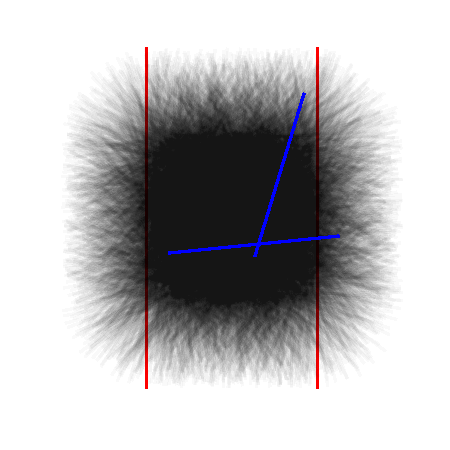
\includegraphics[width=\linewidth]{Rplot02}
  \caption{Ten thousand simulated needle drops overlaid on a graph. The two red lines signify the edges of the floorboards. Two random needle drops are colored blue as examples; one crosses the floorboard edge and the other does not.}
  \label{sim}
\end{marginfigure}

\noindent The classic formulation of this problem uses a needle that is the same width as the floorboards and that is what is used here. The idea is to simulate dropping $10,000$ needles and then count how many cross the edges of the floorboards. In this simulation $6388$ needles overlap an edge so the estimated probability is $ \frac{6388}{10,000} = 63.9\%$. Our estimate is quite close to the true probability which is $63.7\%$.



\section{Estimating $\pi$}

\begin{marginfigure}[.3in]
  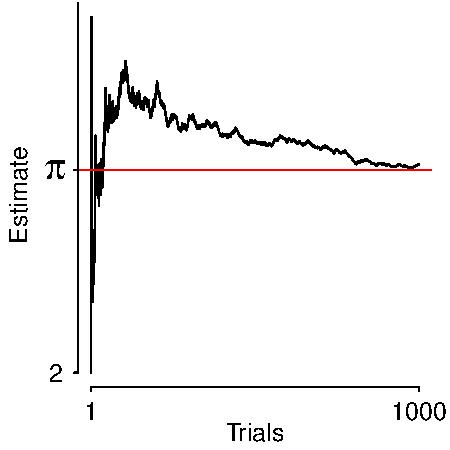
\includegraphics[width=\linewidth]{./graphics/pi.pdf}
  \caption{The estimate of $\pi$ as the number of needles dropped goes from 1 to 1000 compared to the actual value of $\pi$. As can be seen, the estimate is fairly accurate after only about 1000 dropped needles.}
  \label{pi}
\end{marginfigure}

The calculus-based solution states that given needle length ($l$) and floorboard width ($w$), then the probability ($p$) that a needle crosses the edge of a floorboard is $ p=\frac{2l}{w\pi}$. The fact that this formula contains $\pi$ is interesting. It means that this simulation can be used to approximate the value of $\pi$ if we didn't already know it. The graph in Figure \ref{pi} shows the estimated value of $\pi$ as the number of needles dropped goes from $1$ to $1000$. For this particular simulation, the estimated value of $\pi$ is $3.175$.

\end{document}
